\documentclass[11pt]{standalone}
\usepackage{amssymb}
\usepackage{amsmath}
\usepackage[no-math]{fontspec}
\usepackage{unicode-math}
\usepackage{libertinus}
\usepackage{pgf,xcolor}
\usepackage{tikz}
\usetikzlibrary{arrows.meta, backgrounds}
\usepackage{pgfplots}
\pgfplotsset{compat=newest}

\definecolor{my_darkgray}{HTML}{484949}
\definecolor{my_lightgray}{HTML}{F3F4F4}
\definecolor{my_darkblue}{HTML}{005A94}
\definecolor{my_lightblue}{HTML}{CCDEE9}
\definecolor{my_yellow}{HTML}{FFEC7F}
\definecolor{my_red}{HTML}{E60000}
\definecolor{my_orange}{HTML}{E87846}

\begin{document}
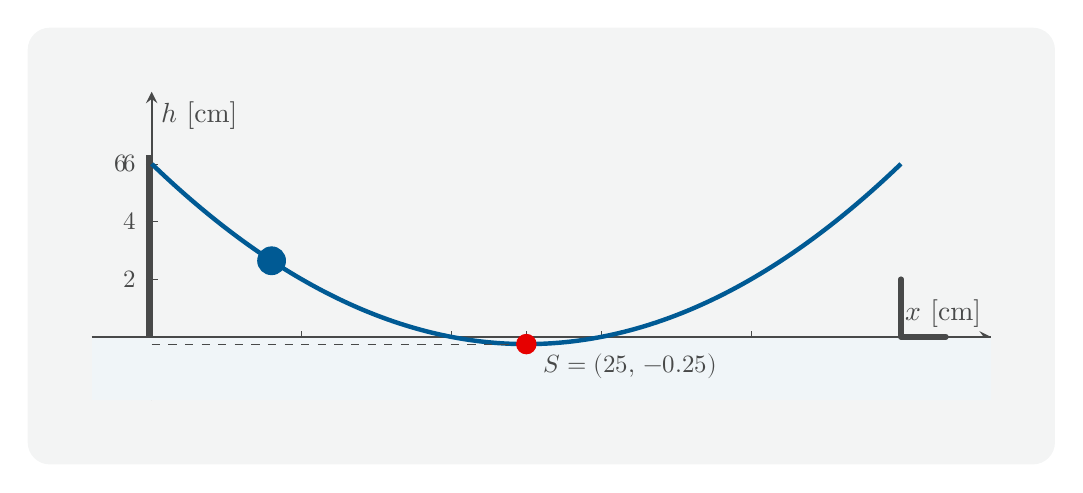
\begin{tikzpicture}[
    show background rectangle,
    background rectangle/.style={fill=my_lightgray, rounded corners=8pt},
    inner frame sep=0.8cm
]
% Track: h(x) = 0.01x^2 - 0.5x + 6,  x in [0, 50],  h in cm.
% Vertex: x=25, h=-0.25 (just below the table surface).
% The track is symmetric: h(0) = h(50) = 6 cm.
% pgfplots axis lines=center places the x-axis naturally at h=0 (the table surface).
\begin{axis}[
    axis lines=center,
    axis line style={thick, my_darkgray},
    tick style={my_darkgray},
    ticklabel style={font=\small, my_darkgray},
    xlabel style={my_darkgray},
    ylabel style={my_darkgray},
    xlabel={$x$~[cm]},
    ylabel={$h$~[cm]},
    height=5.5cm, width=13cm,
    xmin=-4, xmax=56,
    ymin=-2.2, ymax=8.5,
    xtick={0,10,20,25,30,40,50},
    ytick={0,2,4,6},
    % No grid: this is a physical schematic, not a function graph.
    grid=none,
    clip=false,
]

% Shade the region below h=0 (below the table surface) in light blue
% to indicate that the vertex dips below the table.
\fill[my_lightblue!30]
    (axis cs:-4,-2.2) rectangle (axis cs:56,0);

% Table surface: emphasise the h=0 line as a solid surface
\addplot[draw=my_darkgray, thick, domain=-4:56]{0};

% Starting block: thin vertical post at x=0, from table surface to h=6
\fill[my_darkgray] (axis cs:-0.4,0) rectangle (axis cs:0,6.3);

% Finishing block: open catch container at x=50, height 6 cm
\draw[my_darkgray, line width=2pt, line cap=round, line join=round]
    (axis cs:50,2.0) -- (axis cs:50,0) -- (axis cs:53,0);

% Parabolic track: h(x) = 0.01x^2 - 0.5x + 6
\addplot[draw=my_darkblue, samples=300, ultra thick, domain=0:50]
    {0.01*x^2 - 0.5*x + 6};

% Marble at x=8, h = 0.01*64 - 0.5*8 + 6 = 0.64 - 4 + 6 = 2.64
\addplot[only marks, mark=*, mark size=5pt,
         draw=my_darkblue, fill=my_darkblue]
    coordinates{(8, 2.64)};

% Vertex point, marked in red to draw attention
\addplot[only marks, mark=*, mark size=3.5pt,
         draw=my_red, fill=my_red]
    coordinates{(25, -0.25)};

% Dashed lines from vertex to both axes
\draw[dashed, my_darkgray, thin]
    (axis cs:25, 0) -- (axis cs:25, -0.25);
\draw[dashed, my_darkgray, thin]
    (axis cs:0, -0.25) -- (axis cs:25, -0.25);

% Vertex label: placed below and to the right of the point
\node[below right, font=\small, my_darkgray]
    at (axis cs:25.5, -0.25) {$S=(25,\,-0.25)$};

% Height annotation for h=6 on the y-axis
\node[left, font=\small, my_darkgray] at (axis cs:-1, 6) {$6$};

\end{axis}
\end{tikzpicture}
\end{document}
